%!TeX program = xelatex
\documentclass{SYSUReport}
\usepackage{amsmath}
\usepackage{tikz}
\usepackage{booktabs}
\usepackage{multirow}
\usepackage{graphicx}
\usepackage{longtable}
\usepackage{listings}
\usepackage{xcolor}

\lstdefinestyle{mystyle}{
    backgroundcolor=\color{gray!10},
    basicstyle=\ttfamily\small,
    keywordstyle=\color{blue!70!black},
    commentstyle=\color{green!40!black},
    stringstyle=\color{purple!60!black},
    numbers=left,
    numberstyle=\tiny\color{gray},
    frame=single,
    breaklines=true,
    captionpos=b
}

\lstset{style=mystyle}

% 根据个人情况修改
\headl{学号 姓名}
\headr{数据安全和隐私保护}
\lessonTitle{数据安全和隐私保护}
\reportTitle{数据安全和隐私保护实验二：百万富翁问题与不经意传输}
\stuname{姓名}
\stuid{学号}
\inst{网络空间安全学院}
\major{网络空间安全}
\date{2026 年 9 月 24 日}

\begin{document}

\cover
\thispagestyle{empty}
\clearpage

\tableofcontents
\clearpage

\section{实验要求}

\subsection{实验题目}

本次实验围绕隐私计算中的百万富翁问题（Millionaires' Problem）展开，即在两个参与方（比如 Alice 与 Bob）在不直接透露各自财富数值的情况下，判断谁更富有，从而理解隐私保护计算的基本思想。实验包括两个任务：

\begin{enumerate}
    \item 任务一：模拟并实现百万富翁问题的原始求解方案；
    \item 任务二：实现 $n$ 选 1 不经意传输（Oblivious Transfer, OT），并将其用于解决百万富翁问题。
\end{enumerate}

通过编程模拟、结果验证与性能对比，理解安全两方计算的基本思想。

\subsection{实验目标}

\begin{enumerate}
    \item 掌握百万富翁问题的建模方法，理解“仅获知比较结果”的隐私目标。
    \item 理解 OT 对发送方消息和接收方选择的双向保护，并完成基于 OT 的安全比较。
    \item 使用相同数据验证两种方案，分析正确性、通信开销与隐私保护条件。
\end{enumerate}

\subsection{实验要求}

\begin{enumerate}
    \item 使用 Python 完成实验，可调用密码库中的基础运算。两个任务均输出“Alice 更富有”“Bob 更富有”或“双方财富相等”，不得输出对方财富及差值。
    \item 任务一实现基于公钥变换、随机数和交互判断的原始求解方案，说明密钥生成、消息构造、比较判定及相等情况的处理。不得以明文交换、共享变量直接比较或可信第三方代算替代协议。
    \item 任务二先实现 $n$ 选 1 OT（可采用 RSA 或 Diffie-Hellman 体系实现，需说明采用的具体协议与参数），随后使用 OT 处理百万富翁问题。
    \item 在相同设备、输入和可比密码参数下，记录两种方案的正确率、耗时、通信字节数及交互轮数，并对两种方案的隐私性进行分析，列出双方可见信息，解释为何不应泄露未选消息、选择位或额外的财富信息。
    \item 提交完整代码和实验报告，报告需包括实验原理、实验环境、两项任务的实现方式、关键代码解释、测试结果比较和分析。截止时间 10 月 8 日晚 24 时。
\end{enumerate}

\section{实验原理}

\subsection{百万富翁问题}

百万富翁问题由 Andrew Yao 于 1982 年提出，是安全多方计算（Secure Multi-party Computation, MPC）的开端问题。问题描述如下：Alice 和 Bob 是两位百万富翁，各自的财富为 $a$ 和 $b$，他们想知道谁更富，但又不想让对方知道自己的具体财富数值。

百万富翁问题要求双方共同计算比较函数：$a>b$ 时输出 Alice 更富有，$a<b$ 时输出 Bob 更富有，$a=b$ 时输出双方财富相等。允许获知结果本身及其必然推论，但不应获得额外信息。本实验按半诚实模型讨论，即双方遵守协议，但可能分析收到的消息。

\subsection{百万富翁问题原始求解思路}

原始方案利用公钥变换隐藏 Bob 的财富索引：Alice 选取随机数 $x$，用 Bob 的公钥加密得到 $C=x^e \bmod n$ 发送给 Bob；Bob 解密得到 $x$ 后，选取随机素数 $p$，构造模素数序列
\begin{equation}
    z_j = (x - b + j) \bmod p, \qquad j = 1, 2, \ldots, M
\end{equation}
并把序列与 $p$ 发送给 Alice。Alice 计算 $z = (x - a) \bmod p$，检验 $z$ 是否出现在 Bob 的序列中：若 $z \in \{z_j\}$，则存在 $j$ 使 $x-a \equiv x-b+j \pmod p$，即 $j \equiv b-a \pmod p$。由于 $1 \le j \le M$ 且 $p > M$，这等价于 $b > a$，即 $a < b$；否则 $a \ge b$。

原始单次判断只区分 $a \ge b$ 与 $a < b$。为区分相等情况，交换角色、使用全新随机数再比较一次：两次结果均为“$\ge$”时即 $a = b$。实现时须处理模运算边界（$p > M$ 避免余数歧义）、余数间距检验及失败重试（素数生成与随机数选取）。

\subsection{不经意传输}

不经意传输由 Michael Rabin 于 1981 年提出，其核心目标是实现“选择性隐私传输”：发送方持有两条消息 $m_0, m_1$，接收方选择一个索引 $b$ 并只接收到 $m_b$；同时发送方无法得知 $b$，接收方无法获知另一条消息 $m_{1-b}$。本实验实现 $n$ 选 1 的 RSA 版本：

\begin{enumerate}
    \item Sender 生成 RSA 密钥 $(n, e, d)$，选取 $n$ 个互不相同的随机数 $x_1, \ldots, x_n$，把 $(n, e, x_1, \ldots, x_n)$ 发送给 Receiver；
    \item Receiver 选择下标 $\sigma$ 与随机数 $k$，计算 $v = (x_\sigma + k^e) \bmod n$ 并发送给 Sender；
    \item Sender 对每个 $i$ 计算 $k_i = (v - x_i)^d \bmod n$：仅当 $i = \sigma$ 时 $v - x_i = k^e$，故 $k_\sigma = k$，其余 $k_i$ 为随机值；
    \item Sender 发送 $m_i' = (m_i + k_i) \bmod n$；
    \item Receiver 恢复 $m_\sigma = (m_\sigma' - k) \bmod n$。
\end{enumerate}

安全性：Receiver 的 $v$ 被随机数 $k^e$ 盲化，Sender 无法得知 $\sigma$；除选中消息外其余 $k_i$ 为随机值，Receiver 无法恢复未选消息，实现双向保护。

\subsection{基于 OT 的百万富翁问题}

将财富 $a, b$ 写成 $\ell$ 位二进制，从最高位向最低位逐位比较，每一轮使用一次 1-out-of-2 OT 传递比较状态，隐藏 Alice 的选择位 $a_i$。状态编码（相对 Alice）：0 = LESS（更穷），1 = EQUAL（持平），2 = GREATER（更富）。Bob 依据自己的位 $b_i$ 与当前状态构造两个 OT 消息：

\begin{itemize}
    \item 若当前状态为 EQUAL（需要继续比较）：$b_i = 0$ 时 $m_0 = \text{EQUAL}$、$m_1 = \text{GREATER}$；$b_i = 1$ 时 $m_0 = \text{LESS}$、$m_1 = \text{EQUAL}$；
    \item 若当前状态已确定，两个消息均等于当前状态（流程照常执行以隐藏状态）。
\end{itemize}

Alice 通过 OT 选择下标 $a_i$ 拿到 $m_{a_i}$ 得到新的状态。比较结束后状态即最终结果。OT 保证 Bob 不知道 Alice 每轮的选择位，Alice 也无法得知 Bob 的位 $b_i$ 与未选消息。

\section{实验设置}

\begin{table}[htbp]
\centering
\caption{实验软硬件环境}
\label{tab:env}
\begin{tabular}{lll}
\toprule
\textbf{类别} & \textbf{名称} & \textbf{版本 / 说明} \\
\midrule
操作系统 & Windows 11 & 10.0.26200 \\
脚本语言 & Python & 3.9.13（Anaconda）\\
密码运算 & 标准库 pow / random & Miller-Rabin 素性检测自行实现 \\
代码管理 & Git & 2.45.1.windows.1 \\
报告排版 & SYSUReport 模板 & ctexart / XeLaTeX 编译 \\
\bottomrule
\end{tabular}
\end{table}

实验仓库 \texttt{research-week2-millionaire-ot} 的结构如下：

\begin{lstlisting}[caption={实验仓库目录结构}]
research-week2-millionaire-ot/
|-- README.md
|-- code/
|   |-- num_utils.py       # Miller-Rabin 素性检测、随机素数生成
|   |-- millionaire.py     # 任务一：Yao 原始方案
|   |-- ot.py              # 任务二第一部分：n 选 1 OT（RSA）
|   |-- millionaire_ot.py  # 任务二第二部分：基于 OT 的安全比较
|   `-- benchmark.py       # 两方案性能对比
|-- result/                # 运行结果与性能对比
`-- report/                # 实验报告（LaTeX 工程）
\end{lstlisting}

可比密码参数：任务一与任务二均使用 RSA-256 位模数（演示规模），财富范围 $M = 100$，任务二二进制位数 $\ell = 8$（$2^8 = 256 \ge M$）。

\section{实验过程}

\subsection{任务一：百万富翁问题原始求解方案}

\subsubsection{密钥生成与消息构造}

任务一使用 RSA 公钥变换隐藏随机数 $x$。密钥生成通过 Miller-Rabin 素性检测选取两个 256 位随机素数 $p, q$，得到模数 $n = pq$ 与公私钥对；公开指数取 $e = 65537$。核心比较函数如下：

\begin{lstlisting}[language=Python, caption={任务一核心：单次比较（公钥变换 + 模素数序列 + 位置检验）}]
def compare_once(alice_a, bob_b, M, rsa):
    # Alice：随机数 x 用 Bob 公钥加密
    x = random.randrange(2, rsa.n)
    C = rsa.enc(x)                    # C = x^e mod n

    # Bob：解密得到 x，构造模素数序列
    xp = rsa.dec(C)
    p = random_prime(32)
    while p <= 2 * M:                 # p > 2M 保证无余数歧义
        p = random_prime(32)
    seq = [(xp - bob_b + j) % p for j in range(1, M + 1)]

    # Alice：位置检验
    z = (x - alice_a) % p
    found = z in seq                  # 命中 => a < b
    return ('a_lt_b' if found else 'a_ge_b')
\end{lstlisting}

\subsubsection{相等情况的处理}

原始单次判断只区分 $a \ge b$ 与 $a < b$。为区分相等，交换角色并使用全新随机数再比较一次：第一轮判断 $a$ 与 $b$ 的关系，第二轮判断 $b$ 与 $a$ 的关系。两次结果组合得到最终结论（见表 \ref{tab:yresult}）。

\begin{table}[htbp]
\centering
\caption{两次比较结果的组合判定}
\label{tab:yresult}
\begin{tabular}{ccc}
\toprule
\textbf{第一轮（a vs b）} & \textbf{第二轮（b vs a）} & \textbf{最终结论} \\
\midrule
$a \ge b$ & $b \ge a$ & 双方财富相等（$a = b$）\\
$a \ge b$ & $b < a$ & Alice 更富有（$a > b$）\\
$a < b$ & $b \ge a$ & Bob 更富有（$a < b$）\\
\bottomrule
\end{tabular}
\end{table}

\subsubsection{运行结果}

以默认输入 $a = 37, b = 42, M = 100$ 运行，并测试边界用例（$a = b = 50$、$a = 99, b = 0$、$a = 0, b = 99$），结果均正确，如图 \ref{fig:yao} 所示（输出只包含比较结论，不泄露双方财富与差值）。

\begin{figure}[htbp]
    \centering
    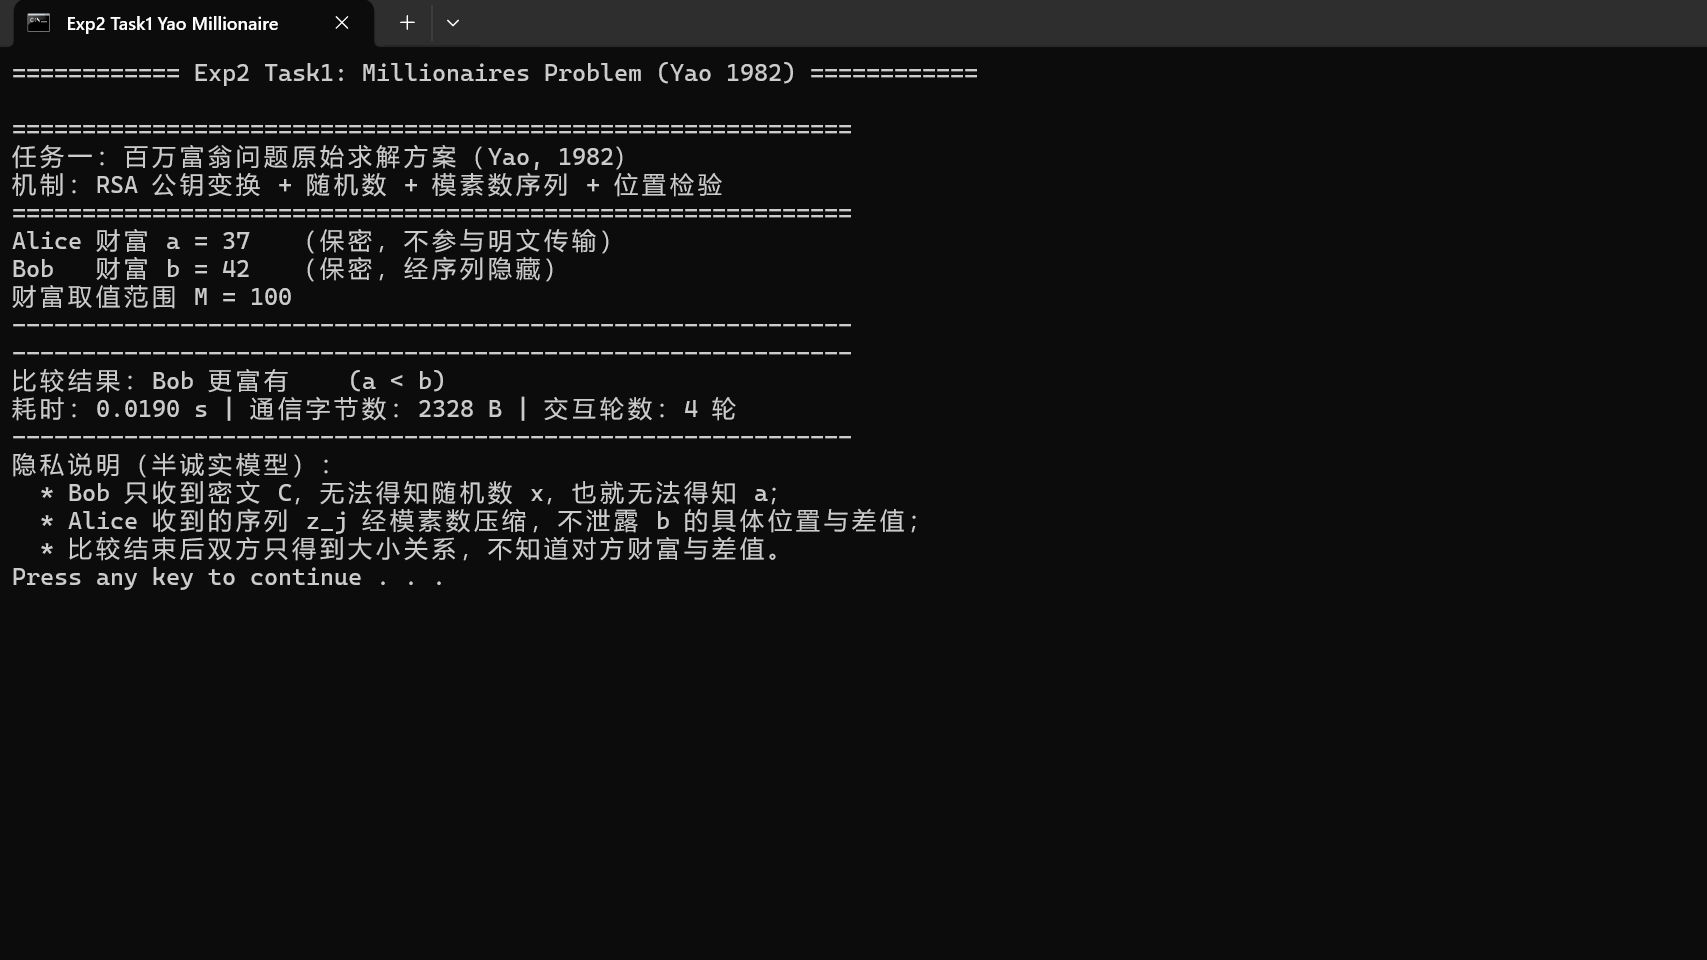
\includegraphics[width=0.95\textwidth]{figures/fig1_yao.png}
    \caption{任务一运行结果（$a=37, b=42$：Bob 更富有）}
    \label{fig:yao}
\end{figure}

\begin{lstlisting}[caption={任务一边界用例验证}]
$ python code/millionaire.py 50 50 100     # 输出：双方财富相等
$ python code/millionaire.py 99 0 100      # 输出：Alice 更富有
$ python code/millionaire.py 0 99 100      # 输出：Bob 更富有
\end{lstlisting}

\subsection{任务二第一部分：n 选 1 不经意传输}

\subsubsection{协议实现}

采用 RSA 体系实现 1-out-of-$n$ OT（Even-Goldreich-Micali 思路推广），参数为 256 位模数。核心代码如下：

\begin{lstlisting}[language=Python, caption={n 选 1 OT 核心（RSA）}]
def ot_n(messages, sigma, rsa_bits=256):
    rsa = RSA(bits=rsa_bits)
    n_mod, e = rsa.n, rsa.e
    # Sender：n 个互不相同的随机盲化数
    blinds = []
    while len(blinds) < len(messages):
        v = random.randrange(2, n_mod - 1)
        if v not in blinds:
            blinds.append(v)
    # Receiver：选择 sigma，随机 k，盲化发送
    k = random.randrange(2, n_mod - 1)
    v_sent = (blinds[sigma] + pow(k, e, n_mod)) % n_mod
    # Sender：解出每个位置的密钥（仅 sigma 处为 k）
    keys = [pow((v_sent - x) % n_mod, rsa.d, n_mod) for x in blinds]
    cipher = [(messages[i] + keys[i]) % n_mod for i in range(len(messages))]
    # Receiver：只恢复自己选中的消息
    received = (cipher[sigma] - k) % n_mod
    return received
\end{lstlisting}

\subsubsection{运行结果}

分别演示 1-out-of-2 与 1-out-of-4 OT，Receiver 均能正确恢复所选消息，且未选消息不可恢复，如图 \ref{fig:ot} 所示。

\begin{figure}[htbp]
    \centering
    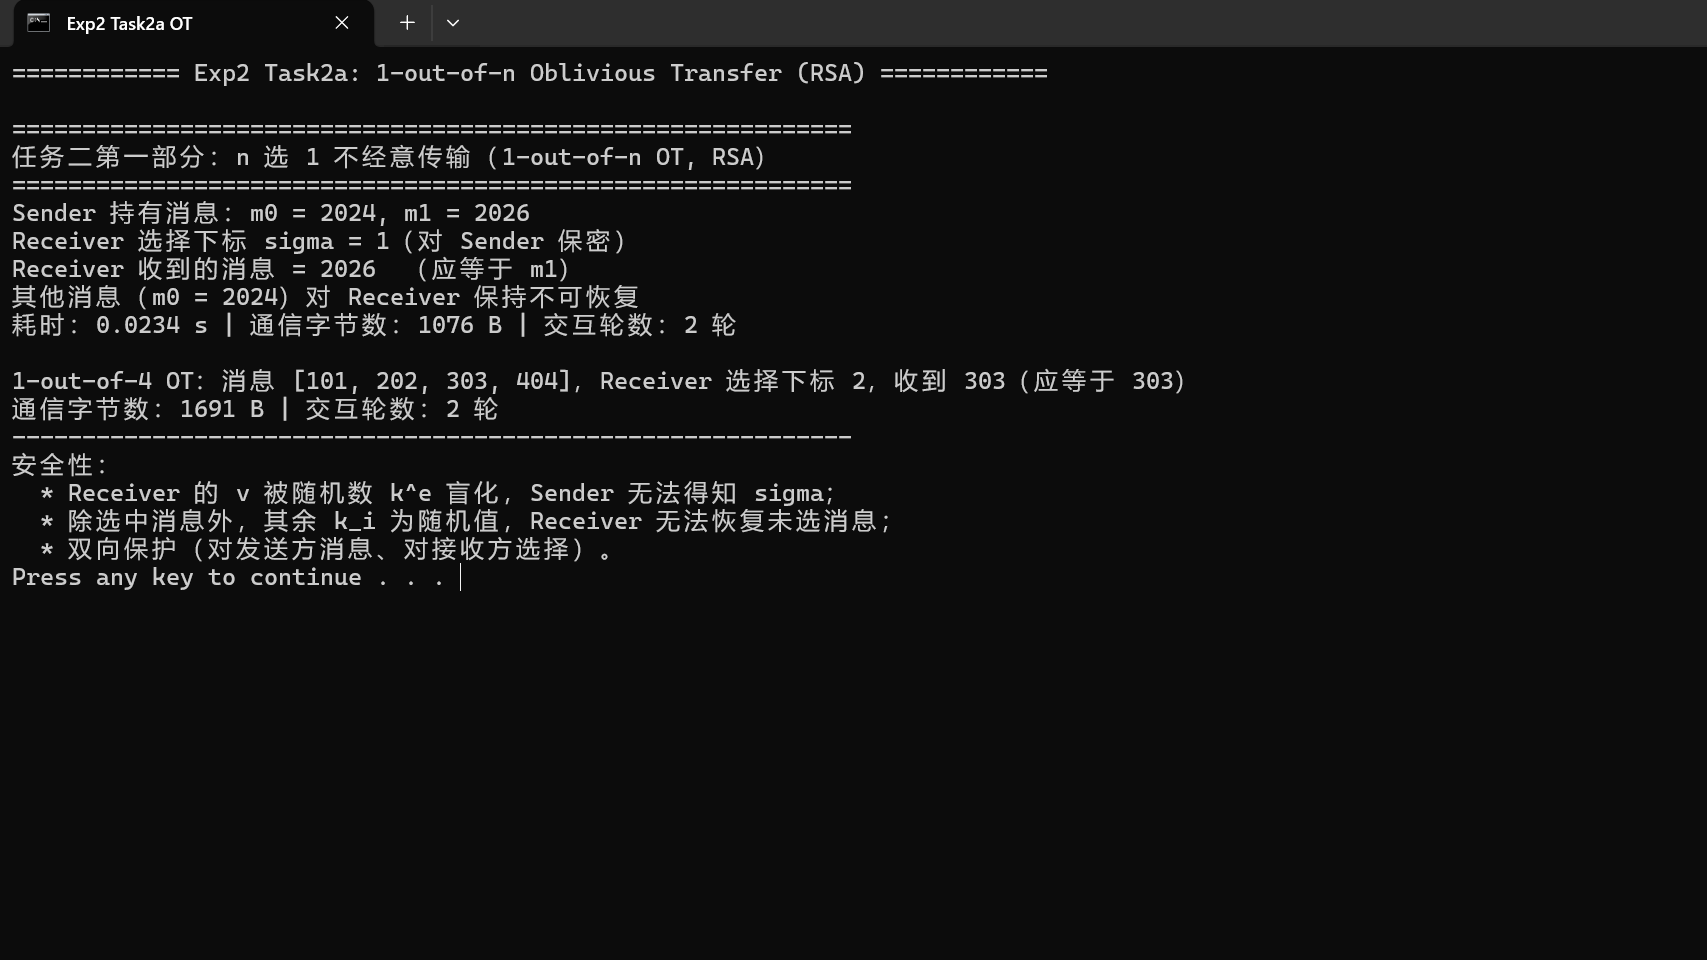
\includegraphics[width=0.95\textwidth]{figures/fig2_ot.png}
    \caption{n 选 1 不经意传输运行结果（1-out-of-2 与 1-out-of-4）}
    \label{fig:ot}
\end{figure}

\subsection{任务二第二部分：基于 OT 的百万富翁问题}

\subsubsection{实现方式}

将财富写成 8 位二进制，从高位到低位逐位比较，每轮调用一次 1-out-of-2 OT 传递比较状态。Bob 构造消息与 Alice 逐位比较的核心逻辑如下：

\begin{lstlisting}[language=Python, caption={基于 OT 的逐位安全比较核心}]
# 状态编码：0 = LESS, 1 = EQUAL, 2 = GREATER（相对 Alice）
def make_messages(b_i, state):
    if state != EQUAL:                # 状态已定，流程照常（隐藏状态）
        return state, state
    if b_i == 0:
        return EQUAL, GREATER         # m0(位0): 持平; m1(位1): 更大
    else:
        return LESS, EQUAL            # m0(位0): 更小; m1(位1): 持平

def secure_compare_ot(a, b, bits):
    state = EQUAL
    for i in range(bits - 1, -1, -1):
        a_i = (a >> i) & 1            # Alice 的选择位（对 Bob 保密）
        b_i = (b >> i) & 1
        m0, m1 = make_messages(b_i, state)
        received, _ = ot_n((m0, m1), a_i)   # Alice 通过 OT 选取
        state = received
    return LABELS[state]
\end{lstlisting}

\subsubsection{运行结果}

以 $a = 37, b = 42, \ell = 8$ 运行并验证边界用例（$a = b = 50$、$a = 99, b = 0$），结果正确，如图 \ref{fig:otcmp} 所示。

\begin{figure}[htbp]
    \centering
    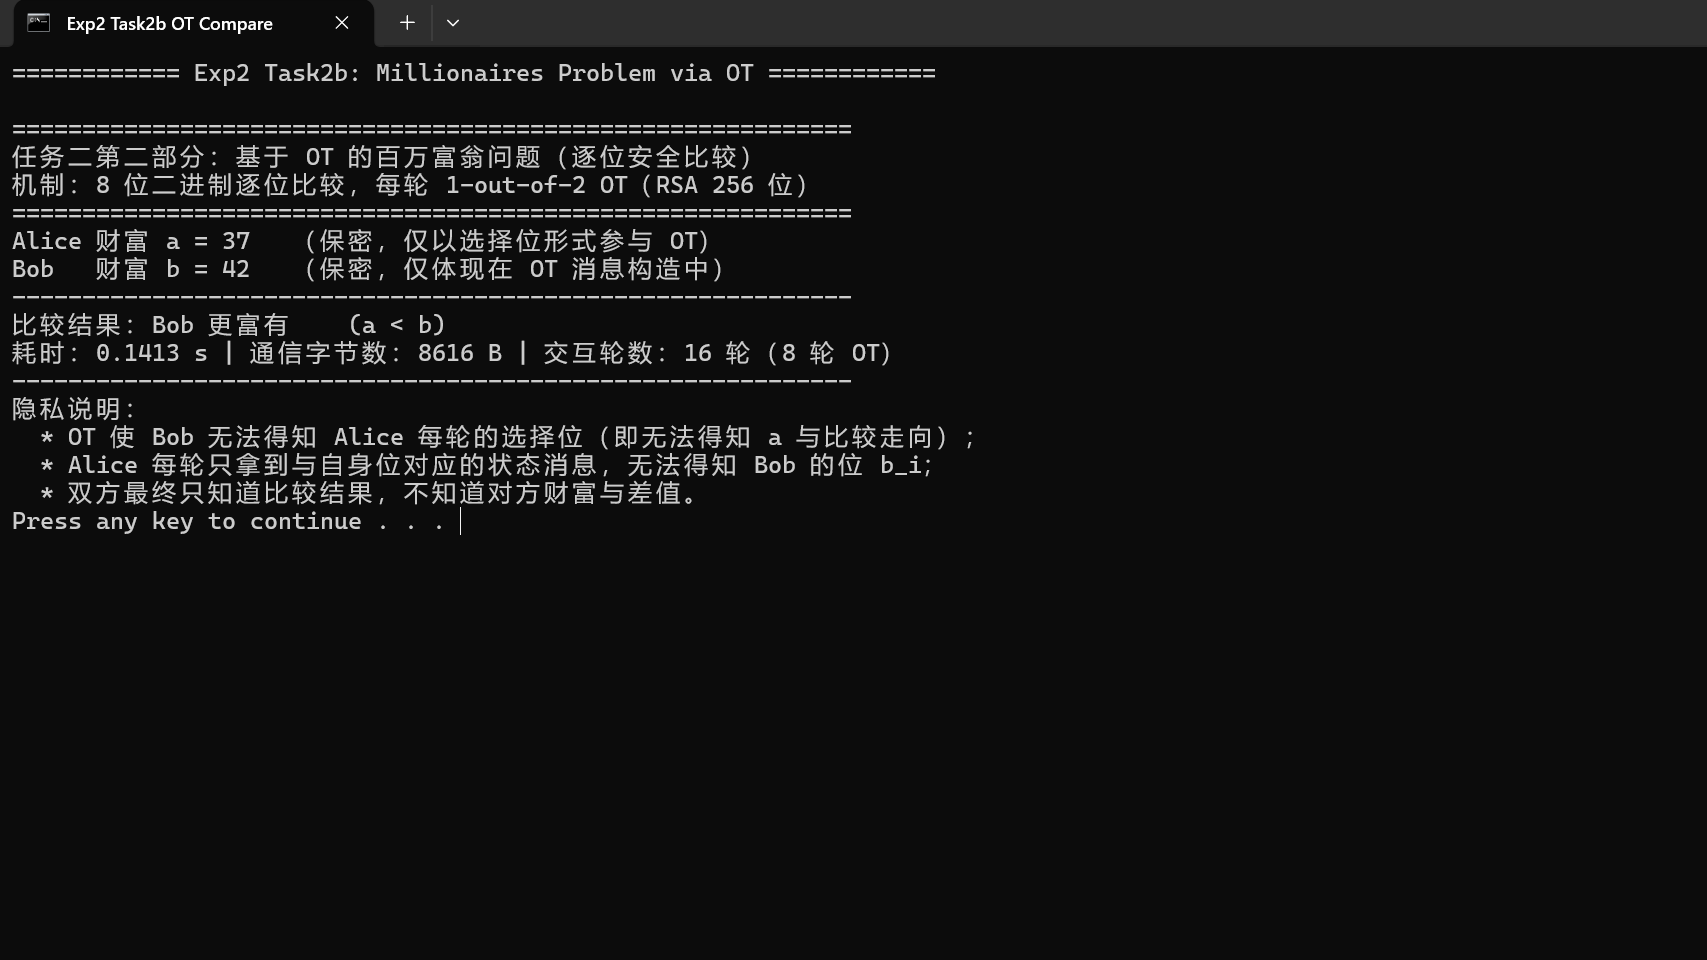
\includegraphics[width=0.95\textwidth]{figures/fig3_otcmp.png}
    \caption{基于 OT 的百万富翁问题运行结果（$a=37, b=42$：Bob 更富有）}
    \label{fig:otcmp}
\end{figure}

\subsection{性能比较与隐私分析}

\subsubsection{性能比较}

在相同设备、相同输入范围（$M = 100$）与可比密码参数（RSA-256）下，对 20 组随机输入运行两种方案，统计结果如表 \ref{tab:bench} 所示，运行界面如图 \ref{fig:bench} 所示。

\begin{table}[htbp]
\centering
\caption{两种方案性能比较（20 组随机输入，范围 $[0, 100)$）}
\label{tab:bench}
\begin{tabular}{lcc}
\toprule
\textbf{指标} & \textbf{任务一：Yao 原始方案} & \textbf{任务二：基于 OT} \\
\midrule
正确率 & 100\% & 100\% \\
平均耗时 (s) & 0.0199 & 0.1353 \\
平均通信 (B) & 2223 & 8620 \\
交互轮数 & 4 & 16 \\
\bottomrule
\end{tabular}
\end{table}

\begin{figure}[htbp]
    \centering
    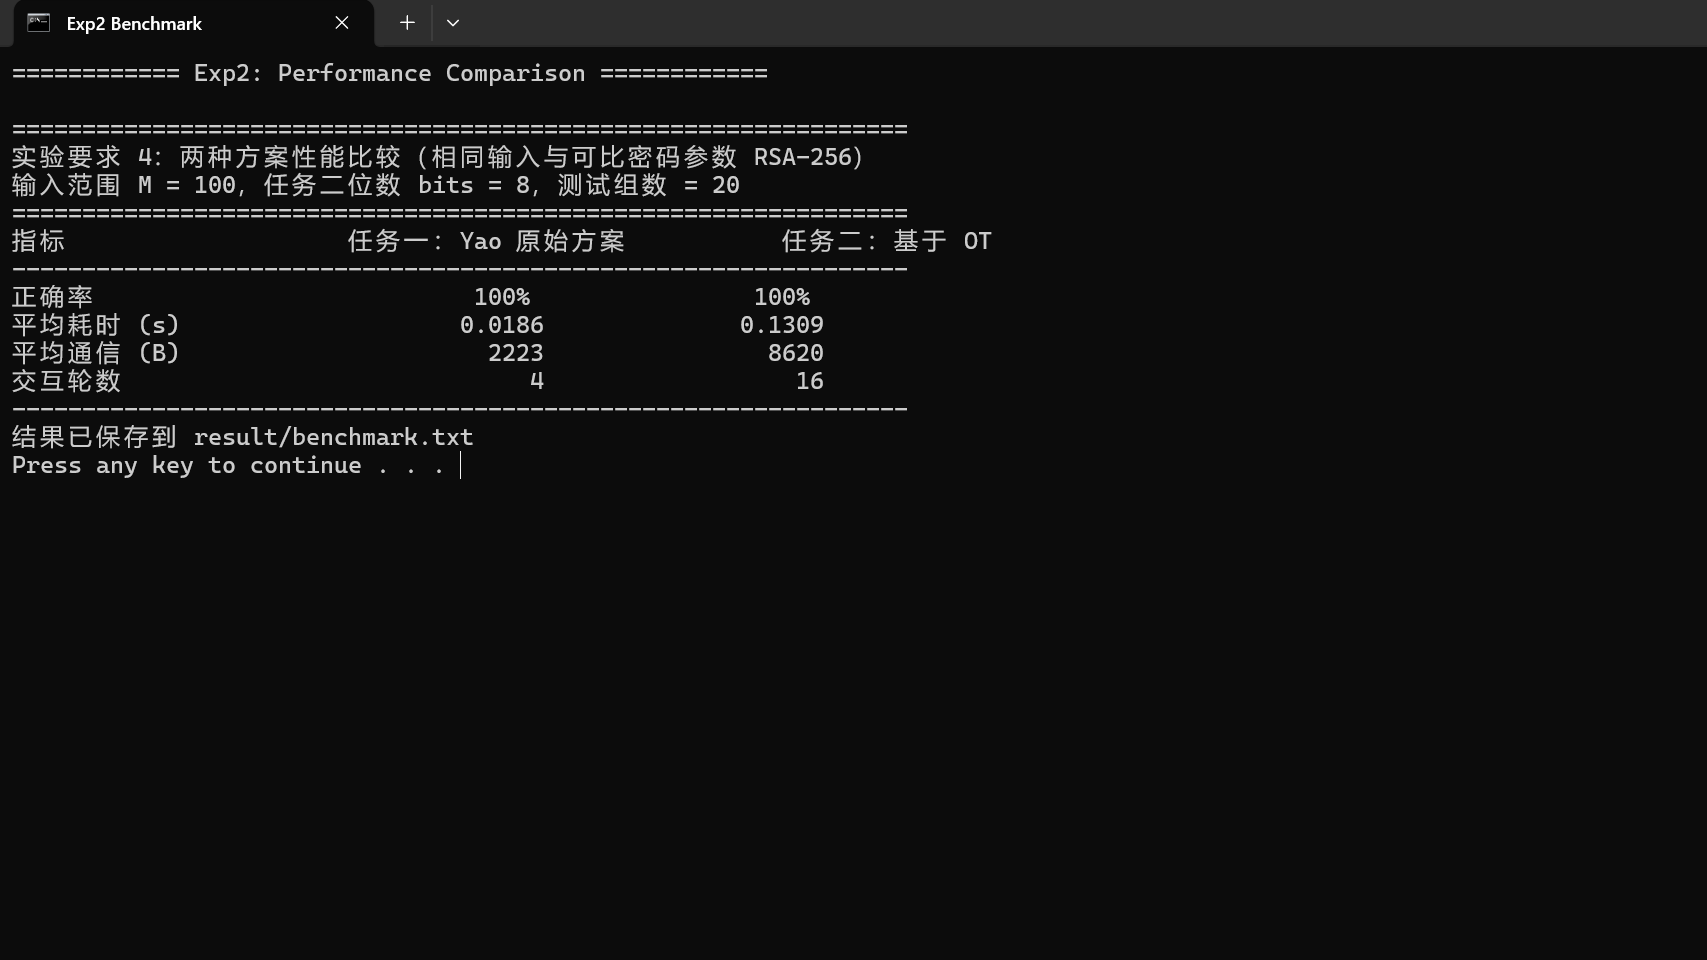
\includegraphics[width=0.95\textwidth]{figures/fig4_bench.png}
    \caption{两方案性能对比运行结果}
    \label{fig:bench}
\end{figure}

结果表明：两种方案在 20 组测试中正确率均为 100\%。任务二耗时约为任务一的 6.8 倍，通信量约为 3.9 倍，交互轮数为 4 倍，主要因为任务二需要 $\ell = 8$ 轮 OT，每轮 OT 都要独立生成 RSA 密钥并完成两轮消息交换。任务一只需 2 次公钥变换比较（共 4 轮），开销更低。耗时会随 RSA 密钥生成的随机性略有波动，但数量级关系稳定。

\subsubsection{隐私分析}

两种方案中双方可见信息与隐私保证如表 \ref{tab:privacy} 所示。

\begin{table}[htbp]
\centering
\caption{双方可见信息与隐私保证（半诚实模型）}
\label{tab:privacy}
\begin{tabular}{p{3.2cm}p{6cm}p{6cm}}
\toprule
 & \textbf{Alice 可见} & \textbf{Bob 可见} \\
\midrule
任务一 & 密文 $C$、模素数序列 $z_j$、比较结果 & 随机数密文 $C$、比较结果 \\
任务二 & 每轮 OT 的两个消息之一、比较结果 & 盲化值 $v$、比较结果 \\
\midrule
\textbf{不可见} & Bob 的财富 $b$、差值 $|a-b|$ & Alice 的财富 $a$、随机数 $x$、每轮选择位 $a_i$ \\
\bottomrule
\end{tabular}
\end{table}

\textbf{为何不应泄露未选消息、选择位或额外财富信息：}

\begin{enumerate}
    \item \textbf{未选消息}：在 OT 中，若 Receiver 能恢复 $m_{1-\sigma}$，则可同时持有两个消息并比对，从而推断 Sender 构造消息时的逻辑（如 $b_i$ 的值），破坏比较协议的隐私性；OT 中其余 $k_i$ 为随机值正是为了防止这一点。
    \item \textbf{选择位}：若 Sender 得知 Receiver 每轮的选择位 $a_i$，结合自身 $b_i$ 即可逐步推断出 Alice 的财富 $a$，甚至最终结果之外的中间信息；OT 通过盲化值 $v$ 隐藏选择位，使 Sender 无法将 $v$ 与某个 $x_i$ 关联。
    \item \textbf{额外财富信息}：协议目标只允许双方获得比较结果及其必然推论。若泄露具体数值或差值，比较结果即可推出对方财富，违背“仅获知比较结果”的隐私目标。任务一中模素数压缩与随机数 $x$ 的作用，任务二中逐位 OT 的作用，都是为了在完成比较的同时不泄露这些额外信息。
\end{enumerate}

\subsection{Git 与 GitHub 使用}

实验代码与报告存放于本地 Git 仓库 \texttt{research-week2-millionaire-ot}，沿用实验一的流程管理版本并推送至 GitHub 远程仓库：

\begin{lstlisting}[caption={Git 初始化的版本管理流程}]
$ git init -b main
$ git add README.md code/ result/ report/
$ git commit -m "add exp2 millionaire problem and oblivious transfer"
$ git remote add github https://github.com/Xu-Rebacca/research-week2-millionaire-ot.git
$ git push -u github main
\end{lstlisting}

推送前使用 \texttt{git status} 与 \texttt{git diff} 核对修改内容，确认无误后提交；最终完整代码与报告已同步至远程仓库，保证实验可复现、可追溯。

\section{实验总结}

通过本次实验，我完成了隐私计算中两个经典问题的建模、实现与对比分析：

\begin{enumerate}
    \item \textbf{百万富翁问题原始方案}：理解了 Yao 1982 原始方案中“公钥变换隐藏随机数 + 模素数序列 + 位置检验”的设计思想，掌握了密钥生成、消息构造、比较判定与相等处理（交换角色再比较一次）的完整流程，并处理了模运算边界与余数歧义问题。
    \item \textbf{不经意传输}：用 RSA 体系实现了 $n$ 选 1 OT，验证了其对发送方消息与接收方选择的双向保护；并将其用于百万富翁问题，通过逐位安全比较完成两方财富比较。
    \item \textbf{性能与隐私分析}：在可比参数下对比了两方案的正确率、耗时、通信量与交互轮数，分析了两方案在效率与轮数上的差异，并从“未选消息、选择位、额外财富信息”三个角度解释了隐私保护的必要性。
    \item \textbf{规范习惯}：全程使用 Git 管理代码与报告并推送远程，报告采用 LaTeX（SYSUReport 模板）撰写，保持“可复现、可追溯、规范保存”的实验习惯。
\end{enumerate}

\end{document}
